\chapter{Die CPP-Referenz am Beispiel der math-library}
\epigraph{Do not worry about your difficulties in Mathematics. I can assure you mine are still greater.}{Albert Einstein}

Zu vielen mathematischen Problemen wie Berechnung der Wurzel oder des Sinus einer Zahl stehen in der math-library \texttt{libm}\footnote{Wie in Abschnitt \ref{sec:Compile} besprochen, muss dem Compiler mitgeteilt werden, wenn eine Bibliothek verwendet wird. Während allgemein von der \emph{math-library} gesprochen wird, heißt die einzubindende Datei leider einfach nur \texttt{m} -- ein unschöner Umstand, mit dem wir leben müssen.} Lösungen bereit. Ich möchte Sie dazu einladen, diese Funktionen selbst zu erkunden. Dazu wird uns die Befehlsreferenz unter \url{https://en.cppreference.com/w/c} dienen. In diesem Kapitel lernen Sie, sich in der Befehlsreferenz zurecht zu finden und nützliche Features selbst zu entdecken.

\section{Überblick über die Seite cppreference.com}
Wenn Sie die Seite \url{https://en.cppreference.com/w/c} besuchen, sollten Sie ein Bild wie in Abbildung \ref{fig:cpp-home} sehen.

\begin{figure}[h!]
	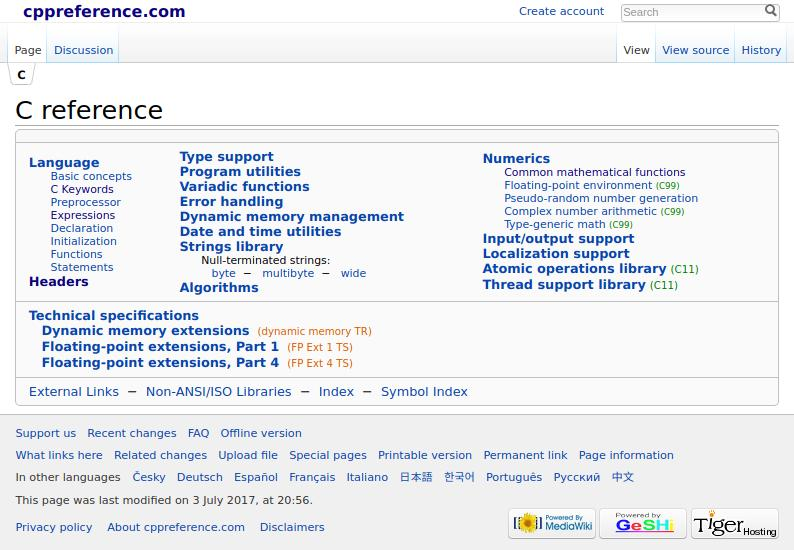
\includegraphics[width=\linewidth]{./gfx/cpp-home}
	\caption{Die Startseite der C-Referenz \url{https://en.cppreference.com/w/c}} \label{fig:cpp-home}
\end{figure}

Der angegebene Link führt Sie auf die \emph{englische} Befehlsreferenz. Übersetzungen in verschiedene andere Sprachen, darunter auch Deutsch, stehen zur Verfügung. In der Regel sind diese aber weit weniger ausführlich und oft unvollständig\footnote{Meiner Erfahrung nach gilt dies generell in der Welt des Programmierens: Nützliche Ressourcen sind oft nur in Englisch verfügbar oder nur in dieser Sprache in vollem Umfang.}. Wenn Sie dennoch mit der deutschen Version arbeiten möchten, finden Sie auf jeder Seite der Referenz am unteren Rand die Zeile \emph{In other languages} und dahinter Links, die sie zu einer entsprechenden Übersetzung führen.

Am rechten oberen Rand befindet sich eine Textbox, in die Sie einen Suchbegriff eingeben können. Die Suche liefert ihnen Ergebnisse zu ihrem Begriff sowie zu \enquote{ähnlichen Ausdrücken}. Die Ergebnisse sind in zwei Spalten sortiert und betreffen die Sprache C++ (links) bzw. C (rechts). In Abbildung \ref{fig:cpp-search} finden Sie das Ergebnis der Suche nach dem Befehl \texttt{printf}. Jede Zeile der Suchergebnisse ist ein Link auf einen Artikel, der den Befehl oder das Konzept erklärt.

\begin{figure}[h!]
	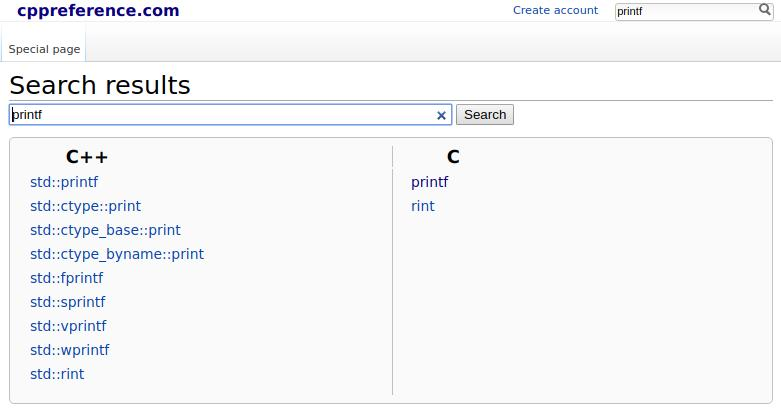
\includegraphics[width=\linewidth]{./gfx/cpp-search}
	\caption{Suchergebnisse in der CPP-Referenz} \label{fig:cpp-search}
\end{figure}

Ein solcher Artikel sieht \idR aus wie in Abbildung \ref{fig:cpp-printf}. Befehle, die sich sehr ähnlich verhalten werden teils zu einem einzelnen Artikel zusammengefasst. Nach der Überschrift finden Sie die Zeile \emph{Defined in header <stdio.h>}, die Ihnen mitteilt, welche \mintinline{c}{#include}s Sie setzen müssen, um den oder die erklärten Befehle in Ihren Programmen nutzen zu können.

Weiter schließt sich eine Syntax-Übersicht an, in der die erwarteten Parameter sowie ihre Datentypen aufgelistet werden. Manche dieser Formen standen nicht in der \enquote{Urform} der Sprache C zur Verfügung. Für solche Features, die erst mit einem bestimmten Standard eingeführt wurden ist in der Referenz in grün das Einführungsdatum bzw. das \enquote{Verfallsdatum} der Form aufgeführt. Ich erinnere Sie daran, dass wir hier den Standard C11 besprechen. In Abschnitt \ref{sec:cpp-article} werden wir anhand eines übersichtlicheren Beispiels auf die Struktur der Artikel eingehen.

\begin{figure}[h!]
	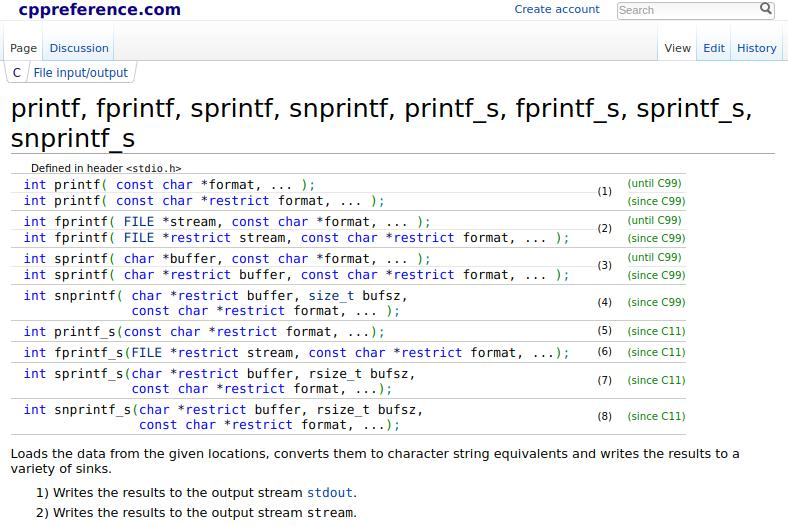
\includegraphics[width=\linewidth]{./gfx/cpp-printf}
	\caption{Anfang des Artikels zu \texttt{printf} auf der CPP-Referenz} \label{fig:cpp-printf}
\end{figure}

\section{Funktionen zu einer Aufgabe finden}
Die Funktionen, die die Sprache C zur Verfügung stellt, sind in thematisch verwandten \emph{Bibliotheken} organisiert. Zu jeder Bibliothek existiert ein \emph{Header}, dessen Name einen Hinweis auf die darin enthaltenen Funktionen gibt. Um Lösungen zu einem gegebenen Problem zu suchen, durchsucht man also am besten die Liste der Header. Diese kann von der Hauptseite aus über den Link \emph{Headers} erreicht werden (siehe Abbildung \ref{fig:cpp-home}, erste Spalte unten). Dieser Link führt Sie zu einer Ansicht wie in Abbildung \ref{fig:cpp-headers}.

\begin{figure}[h!]
	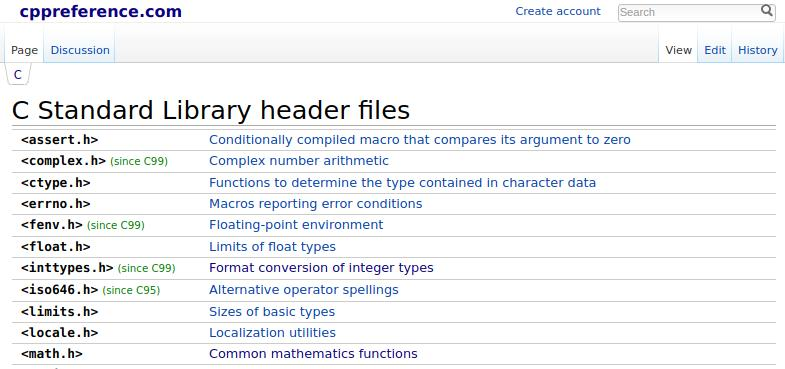
\includegraphics[width=\linewidth]{./gfx/cpp-headers}
	\caption{Liste der Header auf der CPP-Referenz} \label{fig:cpp-headers}
\end{figure}

In diesem Kapitel wollen wir uns mit mathematischen Funktionen befassen; wir klicken daher auf den Link \emph{Common mathematical functions}.

\begin{figure}[h!]
	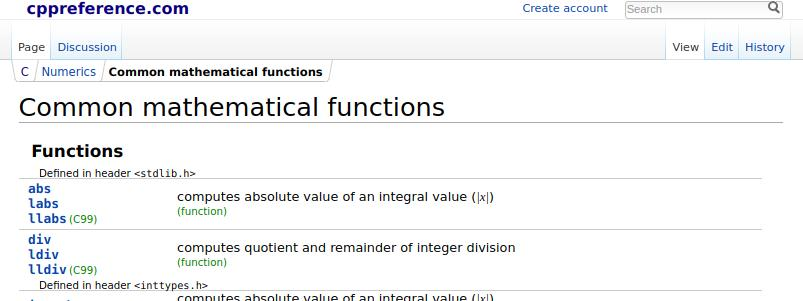
\includegraphics[width=\linewidth]{./gfx/cpp-math}
	\caption{Funktionen der math-library in der CPP-Referenz} \label{fig:cpp-math}
\end{figure}

Wie Sie in Abbildung \ref{fig:cpp-math} sehen, sind die Funktionen in einem ähnlichen Format aufgelistet wie schon die Header. Zu vielen Aufgaben stehen mehrere Funktionen zur Verfügung. Dies hat den Grund, dass die Sprache C \emph{strong-typed} ist, \ie dass Unterschiede zwischen beispielsweise \mintinline{c}{float}- und \mintinline{c}{double}-Werten bestehen. Funktionen, die mit einem \texttt{f} beginnen, berechnen \idR einen \mintinline{c}{float}-Wert; der Anfang \texttt{l} weist auf einen \mintinline{c}{long}-Wert hin und \texttt{ll} erzeugt einen \mintinline{c}{long long}-Wert. Für manche Kontexte sind Ganzzahlen unsinnig; dort weist der Suffix \texttt{l} auf \mintinline{c}{long double} hin. Ist dem Funktionsnamen kein solcher \emph{Präfix} vorangestellt, wird ein \mintinline{c}{double}-Wert berechnet\footnote{Die Benennungs-Logik der C-Standardbibliotheken folgt oft noch veralteten Konventionen, die solche kryptischen Namen hervorbringen. Moderne ProgrammiererInnen bevorzugen \enquote{klare Namen}. Damit auch ältere Code-Teile weiterhin funktionieren musste diese Benennungsregeln fortgeführt werden.}.

Aufgrund des \emph{strong typing} muss auch für die Argumente der Funktionen unterschieden werden. Hier geben die \emph{Suffixe} \texttt{f}, \texttt{l} und \texttt{ll} den Datentyp des Arguments an.

Beispielsweise finden Sie die Funktion \texttt{abs}, die den Absolutbetrag einer \mintinline{c}{double}-Zahl berechnet und als \mintinline{c}{double}-Wert zurückgibt. Daneben ist aber auch \ua die Funktion \texttt{fabsl} aufgelistet, die ebenso den Absolutbetrag einer Zahl berechnet. Die Zahl wird für diese Funktion jedoch als \mintinline{c}{long}-Wert angegeben und das Ergebnis als \mintinline{c}{float} berechnet.

\section{Der Artikel zu \texttt{sqrt}} \label{sec:cpp-article}
\begin{figure}[h!]
	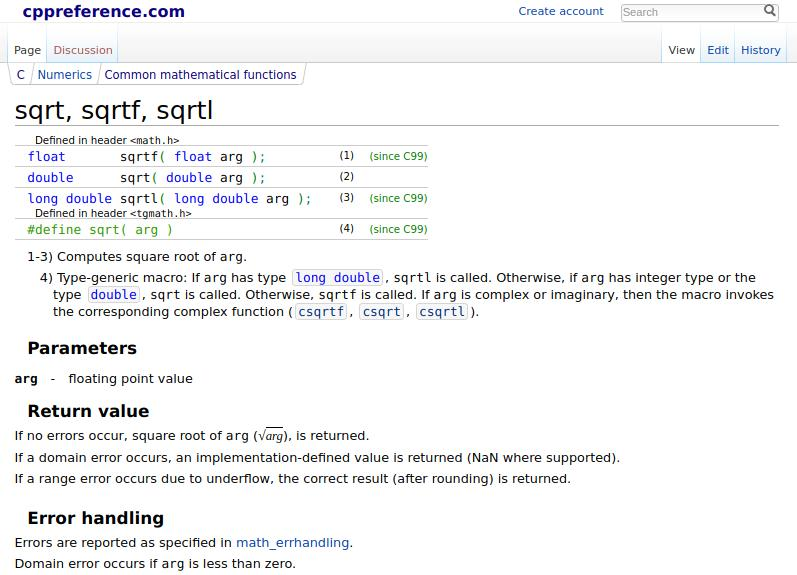
\includegraphics[width=\linewidth]{./gfx/cpp-sqrt}
	\caption{Anfang des Artikels zu \texttt{sqrt} in der CPP-Referenz} \label{fig:cpp-sqrt}
\end{figure}

Abbildung \ref{fig:cpp-sqrt} zeigt den Anfang des Artikels zum Befehl \texttt{sqrt}. Die Zeile \emph{Defined in header <math.h>} weist darauf hin, dass wir \mintinline{c}{#include <math.h>} setzen müssen, um \texttt{sqrt} benutzen zu können. Von dem Befehl stehen drei Varianten zur Verfügung, von denen zwei erst mit dem Standard C99 eingeführt wurden (Punkte 1 bis 3). Weiterhin wurde mit dem Standard C99 ein \emph{Makro} eingeführt (Punkt 4), das wir an dieser Stelle noch nicht bearbeiten wollen. In Kapitel \ref{chp:Preprocessor} besprechen wir die hierzu relevanten Techniken. Für den Moment können Sie den Punkt ignorieren\footnote{Wenn Sie später im Kursverlauf nochmals diesen Artikel in der Referenz lesen, beachten Sie bitte, dass für die Benutzung des Makros der Header \emph{<tgmath.h>} eingebunden werden muss.}.

Unter der tabellarischen Übersicht der im Artikel besprochenen Funktionen finden Sie eine Kurzbeschreibung des Effekts der einzelnen Formen. \emph{1-3) Computes square root of arg.} -- alle hier besprochenen Funktionen berechnen also die Quadratwurzel eines Arguments \texttt{arg}. Der Unterschied ist der Datentyp des Ergebnisses bzw. des Arguments.

Unter \emph{Parameters} finden Sie genauere Erläuterungen zu den Argumenten, die den Funktionen übergeben werden können. Für \texttt{sqrt} ist dies die nüchterne Erklärung, dass \texttt{arg} eine beliebige Fließkommazahl beschreibt. Bei der Funktion \texttt{printf} wird hier etwa aufgelistet, wie ein Formatstring auszusehen hat.

Funktionen berechnen einen Wert, der dann einer anderen Variablen zugewiesen werden kann. Betrachten Sie das folgende Beispiel:

\begin{codebox}[Beispiel: Betrag einer Zahl  mit dem ternären Operator]
\begin{minted}[linenos]{c}
#include <math.h>

int main () {
   double root = sqrt(81.0);
}
\end{minted}
\end{codebox}

Wir benutzen die Funktion \texttt{sqrt} um aus dem \mintinline{c}{double}-Wert \texttt{81.0} die Wurzel zu berechnen und speichern diesen Wert der Wurzel dann in der Variablen \texttt{root}. Dieser berechnete Wert wird als Rückgabewert (\emph{Return Value}) der Funktion bezeichnet.

Der Abschnitt \emph{Return Values} gibt Details zu dem berechneten Wert unter der Annahme verschiedener Szenarios.

Wenn kein Fehler auftritt, wird die Quadratwurzel von \texttt{arg} berechnet. Wie Sie wissen, existiert aber nicht zu jeder Zahl eine Quadratwurzel. So sind negative Werte für \texttt{arg} nicht zulässig -- dies ist gemeint mit \emph{If a domain error occurs}. In diesem Fall hängt das Ergebnis von der Version des Compilers ab (\emph{an implementation-defined value is returned}). In der Regel wird aber ein spezielles Bitmuster erzeugt, das sicher als \enquote{Fehler-Wert} interpretiert werden kann (\emph{NaN where supported} -- \emph{NaN} steht für \emph{Not a Number}, also ein Fehlerwert. Siehe hierzu mehr in Abschnitt \ref{sec:NAN}).

Die letzte Zeile \emph{If a range error occurs due to underflow} beschreibt das Verhalten, wenn der Wert von \texttt{arg} nicht mehr korrekt mit seinem Datentyp abgebildet werden kann (vgl. Abschnitt \ref{sec:Datatypes} im Anhang -- manche Werte sind zu groß oder haben zu viele Nachkommastellen, um beispielsweise als \mintinline{c}{double} exakt abgebildet zu werden). In diesem Fall wird mit einem gerundeten Wert gerechnet.

Unter \emph{Error Handling} werden weitere Details aufgelistet, die das Verhalten von \texttt{sqrt} in \enquote{abnormalen} Situationen beschreiben. Im Allgemeinen ist es nicht nötig, all diese Details im Kopf zu behalten -- dafür ist die Referenz da.

Am Ende der meisten Artikel finden Sie zu jedem Befehl einen Beispiel-Code, der die Anwendung der besprochenen Funktion verdeutlicht, sowie ein Ausgabebeispiel.

\section{Weitere nützliche Funktionen der math-library}
Die folgende Tabelle listet sehr gebräuchliche Funktionen sowie eine Kurzbeschreibung auf. Mit der cpp-Referenz sollten Sie nun dazu in der Lage sein, diese Funktionen in Ihren Programmen anzuwenden.

\begin{table}[h!]
	\newcolumntype{C}{>{\ttfamily\centering\arraybackslash} p{.2\linewidth}}
	\newcolumntype{D}{>{         \centering\arraybackslash} p{.7\linewidth}}
	\rowcolors{1}{white}{chameleonblue2}
\begin{center}
\begin{tabularx}
	{.95\linewidth}
	{CD}
\toprule[1pt]

	\normalfont Funktion  &  Effekt
\tabcrlf

	sqrt  & Quadratwurzel einer Zahl \\
	cbrt  & Kubikwurzel einer Zahl   \\
	pow   & Potenz einer Zahl \texttt{x} zu einem Exponenten \texttt{y}: $x^{y}$ \\
	exp   & Exponentialfunktion      \\
	log   & Natürlicher Logarithmus  \\
	sin   & Sinus                    \\
	cos   & Cosinus                  \\
	tan   & Tangens                  \\
	asin  & Arcussinus               \\
	acos  & Arcuscosinus             \\
	atan  & Arcustangens             \\
	atan2 & Arcustangens mit Unterscheidung der Quadranten \\
	ceil  & Zahl aufrunden           \\
	floor & Zahl abrunden            \\
	trunc & Nachkommaanteil abschneiden \\
	round & Zahl runden              \\

\bottomrule[1pt]
\end{tabularx}
\end{center}
\caption{Gängige Funktionen der math-library}\label{tab:CommonMathFuncs}
\end{table}

\section{Die C++-Referenz}
\begin{plusbox}
Wie die URL der Seite schon vermuten lässt, ist die cpp-Referenz auch ein Verzeichnis der Features von C++. Gehen Sie hierzu von der Adressse \url{https://en.cppreference.com/w/cpp} aus, um Informationen spezifisch zu C++ zu finden.

Sie haben bereits gesehen, dass die Stichwortsuche direkt auf C++-spezifische Artikel verweist. Auf der Startseite der C++-Referenz finden Sie ebenfalls den Punkt \emph{Headers}, von wo Sie auf die spezifischen libraries verwiesen werden. Die bedeutsamsten Bibliotheken sind hier aber schon direkt von der Startseite aus verlinkt.
\end{plusbox}
